\chapter{Design and Solution}

\section{System Structure}

Overall, the whole system includes three parts of hardware modules, naming camera module, user's smartphone, and the server.

Our sign language translating AI system includes six main modules: hand pattern recognition, direction determination, location detection, action detection, word decoder, and text to speech (Figure 4). Firstly, the system continuously captures the hand’s motion, processes it with the hand landmark model, and then puts it into those modules. Each of them has a unique role, and after combining the first four modules’ results (hand pattern, direction, location, and action detection), the word decoder module will take the output data and bring out the corresponding result. Then, the result will show up on the main screen (Figure 16); meanwhile, the phone will speak out that word. In the below sections, we will discuss each module’s role and how it works.

TODO: Replace with new structure

\begin{figure}[H]
  \centering
  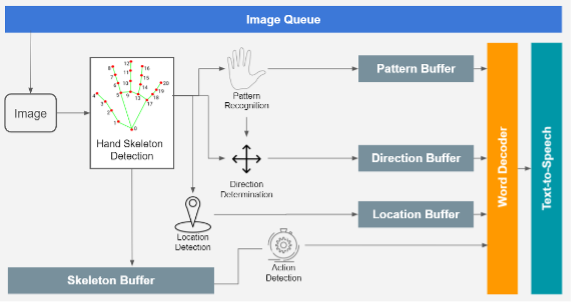
\includegraphics[width=\textwidth]{img/Chap4/OverviewOfTheSystemModules.png}
  \caption{Overview of the system modules}
  \label{fig:Chap4-OverviewOfTheSystemModules}
\end{figure}

\section{Detail Implementation}

\subsection{Hand pattern recognition}

Hand pattern recognition is the first and basic module of this system. While a person with disabilities does signs of sign language, his hands perform a series of different movements, where their hand may be spread out, clenched, or his fingers pointing out at something. Therefore, the role of this module is to recognize the pattern of the hands. Then combining the outcome with other modules, the system can give out the final result.

This module uses the output of the hand landmark model, which is a matrix size of 21. After calculating all the values in that matrix, we get a new matrix representing the distance between those 21 coordinates. Using the distance matrix as the input of CNN [2] with the designed structure (see Figure \ref{fig:Chap4-StructureOfConvolutionalNeuralNetwork}), as seen in Figure \ref{fig:Chap4-OverviewOfTheSystemModules}, will tell us the pattern of the hand at the moment it is captured.

\begin{figure}[H]
  \centering
  
\includegraphics[width=\textwidth]{img/Chap4/StructureOfConvolutionalNeuralNetwork.png}
  \caption{Structure of convolutional neural network}
  \label{fig:Chap4-StructureOfConvolutionalNeuralNetwork}
\end{figure}

\subsection{Direction determination}
FIXME: Thêm các hình ảnh về cách xác định hướng, lấy từ ppt
The directions of the hand include four directions, i.e., right, left, up, down, front, and back. Each hand’s pattern combined with different directions leads to a different meaning. For example, the pattern that points at someone means the word “you”; on the other hand, when we point it to ourselves, it means the word I (see Figure \ref{fig:Chap4-WordYouInSignLanguage} and Figure \ref{fig:Chap4-WordIInSignLanguage}).

\begin{figure}[H]
  \centering
  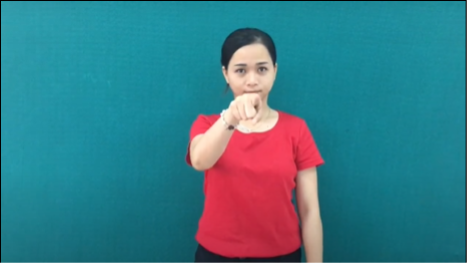
\includegraphics[width=\textwidth]{img/Chap4/WordYouInSignLanguage.png}
  \caption{Word “You” (bạn) in sign language}
  \label{fig:Chap4-WordYouInSignLanguage}
\end{figure}

\begin{figure}[H]
  \centering
  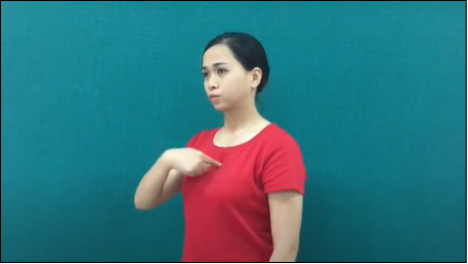
\includegraphics[width=\textwidth]{img/Chap4/WordIInSignLanguage.png}
  \caption{Word “I” (tôi) in sign language}
  \label{fig:Chap4-WordIInSignLanguage}
\end{figure}

To determine the hand’s direction, we use the hand landmark model provided in MediaPipe (see section 2 TK). The inception here is that we calculate the distance between the tip of the index finger and the wrist (called TK), then project it to the axis Ox, Oy, Oz, respectively. After that, we take each of those coordinates and compare them with the others. Finally, the one with the immense value will tell which axis the hand is on; besides, with the direction from the wrist to the tip of the index finger projected on that corresponding axis, we will know which direction the hand is.

For instance, a hand is known to be pointing toward the left direction. The value of the distance, when projected on the axis Ox, will be the biggest one among the three projected values. Then, calculate the vector drawn from the wrist to the tip of the index finger; we will know the direction of the hand itself.

\subsection{Location detection}
FIXME: Giới thiệu previous approach về sử dụng độ zoom, các khó khăn
FIXME: Thêm các hình ảnh về cảm biến sóng âm, các thông số, tại sao lại sử dụng, sử dụng như thế nào

Locations of hand vary, is the hand put at forehead, mouth or the chest level, and so on. Every hand pattern that goes with every location will result in different words. Nevertheless, it is hard for the AI to know the hand’s location with only one camera, and its view is from above (see Figure \ref{fig:Chap4-ViewFromCamera}). However, we came up with some solutions to this issue.

Firstly, we will take pictures of the hand and calculate the size of the hand in every frame in order to know whether that hand is getting bigger or smaller. Hence, if that hand is smaller than before, it means the hand is getting far away from the camera, and its location is somewhere at the chest level or the stomach level.

\begin{figure}[H]
  \centering
  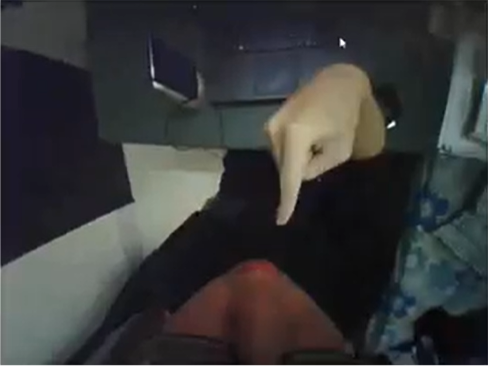
\includegraphics[width=\textwidth]{img/Chap4/ViewFromCamera.png}
  \caption{View from the camera module}
  \label{fig:Chap4-ViewFromCamera}
\end{figure}

Nonetheless, the above solution still has an issue: every man’s hand has a different size, and the system does not know the correct position of the hand. Therefore, another solution is to use a wide-angle camera and set it away from the forehead. With this solution, the camera can have a much broader view. However, since we only have a normal-angle camera, we could not try out this solution and confirm its suitability.

\subsection{ Design}
  TODO: Trình bày các thiết kế hiện có và các chức năng phụ

\subsection{Word decoder}

TODO:   Previous approach 
      [...] How to map word ?
TODO:   New approach
      [] Punish function
      [] Using beam search
      [] CTC decode
      [] Flow
      [] Expected result
      [] Difficult and proposed solution

  \subsection{ Previous approach}
    TODO: With previous approach, trình bày hướng đi
    cũ của module này, khi còn sử dụng module action
    detection, lúc này, một word sẽ được trình bày dưới
    dạng 4 module cơ bản (pattern, location, direction, action),
    khi đó, nhiệm vụ của chúng ta là tìm trong cơ sở dữ liệu, từ nào
    tương ứng với các kết quả thu được từ 4 module trên, khi đó
    ta sẽ thu được từ vựng.
    TODO: Insert image represent the way to map word with 4 module
                              [p,l,d,a]
                        Map   [p1,l1,d1,a1]
              [p,l,d,a] ----> [p2,l2,d2,a2] ---> word
                              [p3,l3,d3,a3]
              Input             database

    Sau khi map được từ vựng, chúng ta sẽ xuất từ vựng đó lên màn hình

    \subsection{ New approach with CTC beam search decode }
      \subsubsection{ Introduction to handstate }
      \subsubsection{ Punish function to get matrix which is input of beam search }
        TODO: Why we need punish -> Do trước khi vào module beam search, ta cần một matrix biểu diễn sự tương quan giữa các output nhận được từ các component và các dữ liệu trong database
        TODO: how to perform -> Trình bày cách đánh giá như thế nào, cách trừ điểm và các phương châm đánh giá
        TODO: Sau khi punish dùng hàm softmax để chuyển các giá trị về dạng xác suất
      \subsubsection{ Using beam search and CTC decode to map word }
        TODO: Trình bày cách sử dụng beamsearch để tìm các cặp bộ 3
        TODO: Image beamsearch (get from ppt)
        TODO: Example
        TODO: Áp dụng CTC để handle một số trường hợp
        TODO: Các khó khăn gặp phải và hướng giải quết

\subsection{Text to speech}

Besides displaying the translated sign language in text form, we included a text-to-speech module to know the result without looking into the screen. This module makes use of a free API provided by Google, named Text-to-Speech [4]. It converts arbitrary strings, words, and sentences into the sound of a person speaking the same things.
